\documentclass[11pt]{article}
\usepackage[utf8]{inputenc}
\usepackage[T1]{fontenc}
\usepackage{graphicx}
\usepackage[export]{adjustbox}
\graphicspath{ {./images/} }
\usepackage{amsmath}
\usepackage{amsfonts}
\usepackage{amssymb}
\usepackage[version=4]{mhchem}
\usepackage{stmaryrd}

\begin{document}
The LP and GP Relationship Life Cycle

Most PE funds have a finite life of very roughly 10 years. A key aspect of PE fund investing is that successful management teams that serve as GPs of PE funds oversee multiple funds through time. Further, satisfied institutional investors in those funds seek to invest in the new funds being offered by successful GPs. This lesson discusses this practice in detail.

\section*{The Relationship between LPs and GPs in Private Equity}
The LP-GP relationship is a classic principal-agent relationship, which, because information in PE markets is incomplete and highly asymmetric, has evolved to address the problems of moral hazard and conflict of interest. There is a symbiotic relationship between LPs and GPs. An LP's investment strategy is built around a number of relationships with GPs, who focus on specific segments (such as stages or sectors) of the market. This specialized focus can often limit the scalability of a particular fund, especially in the case of VC, in which LPs may find it difficult to identify and access additional fund managers of comparable quality.

GPs, for their part, want financially strong, dependable, knowledgeable, and long-term LPs. LPs should have industry expertise and familiarity with the nuts and bolts (particularly valuations and benchmarking) of the PE business. Adverse selection exists in the PE market: Poor-quality GPs, be they lacking experience or falling into decline, will court inexperienced LPs. Because of poor results, both will eventually exit the market.

To maintain continuous investment in new portfolio companies, GPs need to raise new funds as soon as the capital from their latest active fund is fully invested (or reserved for follow-on investments), that is, about every three to five years. Thus, relationships between LPs and GPs follow a life cycle and are forged through various rounds of investment, eventually resulting in a virtuous circle of growing experience and fund size.

Anecdotal evidence suggests that experienced market players profit from these relationships over protracted periods of time. Initially, criteria are very stringent, and fund managers usually cannot get rich through their first funds. However, a favorable track record is an asset in itself. For more reputable funds, fundraising is less costly. To minimize their expenses, fund managers generally turn first to those who invested in their previous partnership, provided that the fund's performance was satisfactory. While it is easy to see how fund managers benefit from a loyal and reliable investor community, these long-term relationships can also be advantageous for LPs. In the opaque PE market, the search for and due diligence of funds is a costly exercise, and LPs often prefer familiar fund managers to unproven investment proposals.

Such long-term relationships may provide access to a quality deal flow of co-investment opportunities in portfolio companies within an established framework. It is especially desirable for an investor to hold on to good fund managers, as the best teams will have an established investor base (i.e., a set of established and loyal clients), which may eliminate the need to seek out new funding sources to the detriment of adding value to the portfolio companies when making new investments or exits. There is likely to be better planning, as LPs make clear their intentions to participate in follow-on funds. As LPs form a network, even if they do not have the means to continue, they often refer other investors to a good team. Predictable closings put money to work more efficiently.

\section*{The Three Phases in the Relationship between LPs and GPs}
The life cycle of the GP-LP relationship (see Fund Manager-Investor Relationship Life Cycle exhibit below) focuses on the long-term pattern of GPs as they create multiple funds through time. The GP-LP life cycle can be divided into three phases: (1) entry and establish (the phase involving the initial funds); (2) build and harvest (or grow and compete), the phase in which the funds thrive and grow; and (3) the three potential outcomes: decline (lost competitiveness), exit (gave up or made it), or transition to new managers (spinouts).

\begin{center}
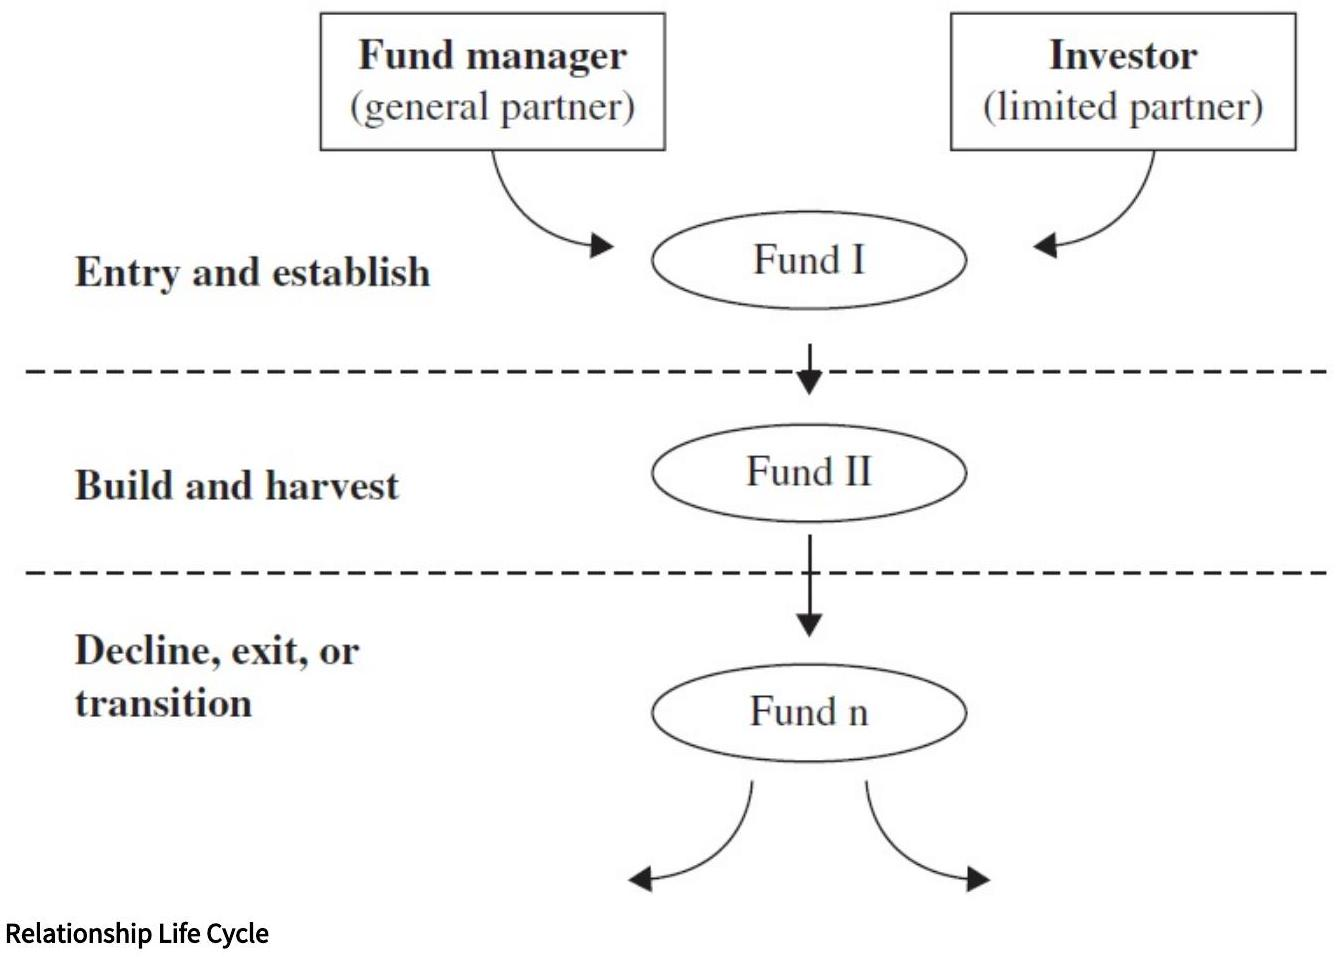
\includegraphics[max width=\textwidth]{2024_04_10_f548a09b7062d16b2a5eg-2}
\end{center}

Fund Manager-Investor Relationship Life Cycle

The main differences between these phases are summarized in the GP-LP Relationship Life Cycle Model exhibit below.

During the entry and establish phase, substantial entry barriers into the PE market exist for both GPs and LPs. Lacking a verifiable track record, new teams find it difficult to raise their first fund. Furthermore, analysis of historical benchmark data supports the hypothesis that new teams suffer from higher mortality than do established or institutional-quality fund managers. First-time funds note the importance of differentiation or innovation as applied to fundraising and thus often pursue specialized investment strategies.

GP-LP Relationship Life Cycle Model

\begin{center}
\begin{tabular}{|llll|}
\hline
Fund's characteristics & Entry and establish & Build and harvest & Decline or exit \\
\hline
Investment strategy & Differentiation & "Star" brand & Unexciting \\
Fundraising & Difficult fundraising & Loyal limited partner base & Limited partners leave and are replaced by other types of investors \\
 &  &  & (secondary plays, new entrants in market) \\
Performance & Unknown: either "top" or "out" & Likely "top" performer & Not "top" but consistent performer \\
Size & Fund is too small & Fund size is right & Fund size too large/too many funds \\
Economies of scale & Fund too small to get rich & Best alignment of interests & Senior managers "made it" \\
Management team & Management team forming & Management team performing & Succession issues, spinouts \\
\hline
\end{tabular}
\end{center}

New LPs also face entry barriers, suffering the initial informational disadvantages that make it extremely difficult to identify or gain access to the best managers, particularly when those funds are oversubscribed. For LPs, it takes the disciplined execution of a long-term investment strategy to build up a portfolio of funds that gives attractive and sustainable returns.

Since investors are mainly interested in the cash returned, the fund manager-investor relationship tends to be relatively stable throughout the build and harvest phase. Lerner and Schoar present evidence on the high degree of continuity in the investors of successive funds, and the ability of sophisticated investors to anticipate funds that will have poor subsequent performance. ${ }^{1}$ Josh Lerner and Antoinette Schoar, "The Illiquidity Puzzle: Theory and Evidence from Private Equity," Journal of Financial Economics 72, no. 1 (2004): 3-40.

It is an oversimplification to assume that investors invest only in top performers and that below-average funds are unable to continue. As in most relationships, there is a certain degree of tolerance for mistakes and failures, at least over a limited period of time. It is clear that there are limits to disappointing results, but all things being equal, investors will tend to go with fund managers they already know or who have been referred to them through their network, even if the fund's performance has been subpar at times.

Eventually, the relationship ends in the decline, exit, or transition (spinout) phase. Not surprisingly, the terms marriage and divorce are often used in the context of relationships between fund managers and their investors. A gradual decline may occur either as a result of past successes, which potentially decrease the financial motivation of senior fund managers, or due to an improperly planned succession, which leads to the departure of middle management. In addition, the LPs may eventually end the relationship if they lose confidence or trust in the team (for example, if the team becomes arrogant or fails to deliver). Some LPs do not invest in follow-on funds and may be replaced by less deep-pocketed or experienced investors, or by secondary investors who choose to invest as a one-off financial play.


\end{document}